\chapter{Requirements Engineering}
\begin{figure}[H]
    \centering
    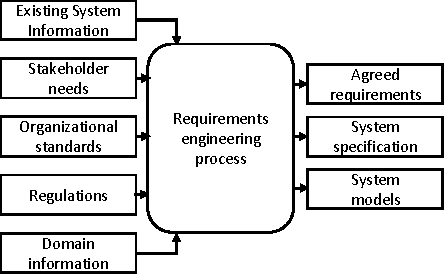
\includegraphics[scale=1.3]{img/RequirementInformationStream.pdf}
    \caption[Information flow in Requirements Engineering]{Information flow in Requirement Engineering (\protect\cite[28]{Kotonya.2000})}
    \label{fig:reqFlow}
\end{figure}
Engineering requirements for a to-be system requires a large diversity of input information (cf. \Cref{fig:reqFlow}). The goals of \textit{Requirement Engineering} is to produce a set of requirements fitting to a modeled and specified system \parencite[cf.][262]{Pohl.2007}. \textit{Requirement Engineering} implies a repetitive and systematic approach to generate complete, relevant, consistent etc. requirements \parencite[5]{Sommerville.2000}. This approach includes the generation and management of requirements \parencite[262]{Pohl.2007}.
\paragraph*{}
Information sources for \textit{Requirements Engineering} include:
\paragraph*{Existing System Information} include all information about systems to be interacted with, as well as a potential legacy system \parencite[cf.][28]{Kotonya.2000}.
\paragraph*{Stakeholder needs} Stakeholders of a system are people or institutions that have some kind of direct or indirect causal relation with the system \parencite[cf.][8]{Sommerville.2000}. This may be users, developers, sponsors, customers, employees and many more. Each stakeholder has some needs for the system, may it be politically in the organization, support of work, legal determinations etc. \parencites[cf.][28]{Kotonya.2000}[cf.][350-351]{Lauesen.2008}
\paragraph*{Organizational standards} Conformaty assurance within one company by regulating system development, quality management etc. \parencite[28]{Kotonya.2000}
\paragraph*{Regulations}
\section{Requirement Engineering Process} 
\begin{figure}[H]
    \centering
    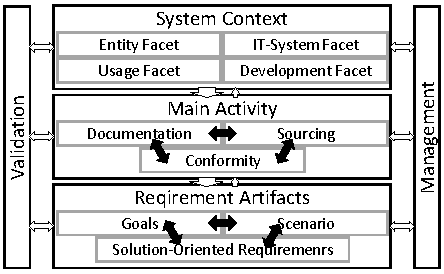
\includegraphics[scale=1.5]{img/ReqAnFrameWork.pdf}
    \caption[Framework for Requirements Engineering]{Framework for Requirements Engineering (own illustration based on \protect\cite[41]{Pohl.2007})}
    \label{fig:reqFramework}
\end{figure}
The \textit{Requirements Engineering Framework} by \textcite{Pohl.2007} defines the structural approach of filling the gap between input information and the vision and goals of a desired output (cf. \Cref{fig:reqFramework}). It analyzes the input information into four different facet of the system context: the entities, the IT-system, the usage and the development of desired application. The structured information is processed in three main activities (documentation, sourcing and confirmation), which lead to the requirement artifacts which represent the vision and goals of the product. \parencite[][38-39]{Pohl.2007}
\subsection{System Context}
Defining the boundary of \textit{System Context} is essential for successful \textir{Requirements Engineering}. It reflects in what way the desired outcome is related to objects - no matter whether physical or not \parencite[55]{Pohl.2007}. \textit{Context Diagrams} - as an example for visual \textit{System Context} representation - treat the system \say{as a black box surrounded by user groups and external systems with which it communicates} \parencite[76]{Lauesen.2008}. The \textit{System Context} represents the environment of a system, which is relevant for requirement analysis \parencite[55]{Pohl.2007}. The boundaries of the system context must be defined to scope out the not relevant part of the environment \parencite[55-56]{Pohl.2007}. The four facets for structuring input information of the system context of \textcite{Pohl.2007} are the following:
\paragraph*{Entity Facet} 
Entities are the digital representation of real world objects and their traits. This can include people such as users and subjects, physical objects such as assets, immaterial objects such as measurements, and processes. Important stakeholders are  professionals for the technical view and legal advisor and data security officials ensuring compliance. \parencite[cf.][70-71]{Pohl.2007}
\paragraph*{IT-System Facet}
The systemic facet of the \textit{System Context} is considering interface requirements to other technical systems such as the underlying hardware or systems the desired product must or may interchange data with \parencite[cf.][192]{Kotonya.2000}. Relevant stakeholders are architects, developers, test and maintenance professionals of the context systems, not the desired system \parencite[cf.][72]{Pohl.2007}.
\paragraph*{Usage Facet} Deals with the demand by direct and indirect users for the system. User is this sense are people and systems having a direct interface with the desired product or are somehow impacting the interaction with the desired product or impact the usage of the system. \parencite[cf.][75-77]{Pohl.2007}
\paragraph*{Development Facet}
This facet regards all information about the development process. Stakeholders and sources for this facet mainly are people involved with the design, implementation and controlling of the development process, guidelines, standards and norms for development, and best practices and project reports. \parencite[cf.][79]{Pohl.2007}
\subsection{Main Activity}

\subsubsection*{Documentation}
\subsubsection*{Sourcing}
\subsubsection*{Conformity}
